\begin{figure}
    \centering
    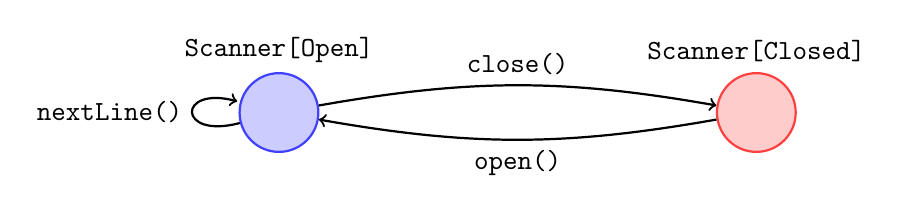
\begin{tikzpicture}
        \tikzstyle{open-file}=[circle, thick, draw=blue!75, fill=blue!20, minimum size=10mm]
        \tikzstyle{closed-file}=[circle, thick, draw=red!75, fill=red!20, minimum size=10mm]
        \tikzstyle{transition} = [->, thick];

        % \draw (0, 0) grid (\textwidth, 2);
        \node[open-file, label=above:\texttt{Scanner[Open]}] (open-file) at (0.25\textwidth, 1) {};
        \node[closed-file, label=above:\texttt{Scanner[Closed]}] (closed-file) at (0.75\textwidth, 1) {};
        \draw[transition]
        (open-file)
        edge[out=10, in=170] node[above] {\texttt{close()}}
        (closed-file) ;
        \draw[transition]
        (closed-file)
        edge[out=-170, in=-10] node[below] {\texttt{open()}}
        (open-file);
        \draw[transition]
        (open-file)
        edge[loop left] node {\texttt{nextLine()}}
        (open-file);
    \end{tikzpicture}
    \caption{The \keyword{Scanner} typestate automata, based on \autoref{lst:java-scanner-typestate}.}
    \label{fig:file-automata}
\end{figure}